\documentclass[12pt]{article}
\usepackage{pslatex} % Font Times New Roman

\usepackage{amsmath,amssymb,amsfonts,amsthm,fancyhdr,lastpage}
\usepackage{makeidx, graphicx}

\setlength{\textheight}{9.0in}
\setlength{\topmargin}{-.5in}
\setlength{\textwidth}{6.5in}
\setlength{\oddsidemargin}{-.0in}
\setlength{\parskip}{6pt}


\renewcommand{\headrulewidth}{0pt}
\setlength{\headsep}{.35in}
\addtolength{\headheight}{2.5pt} 

\usepackage{graphicx}

\begin{document}

\title{Comparative Analysis of Methods for Obtaining Realistic Graphs from Kekule Cells}
\author{Aaron Germuth and Alex Aravind \\\\  
Department of Computer Science \\
University of Northern British Columbia \\
E-mail: (germuth,csalex)@unbc.ca}
\maketitle


\begin{abstract}

The switching behavior seen in conjugated hydrocarbons may be used for molecular electronics. Hesselink has previously classified all possible switching behaviours into Kekule cells \cite{H13}, and found matching graphs. This study compares the use of 4 different methods for obtaining graphs that match each Kekule cell of rank \textless  7. However, we impose multiple restrictions onto our graphs to ensure they only resemble realistic molecules. Out of the 214 cells in rank 7, 32 could be obtained with graph modification, 44 with template molecules, 70 with a genetic algorithm, and 135 with the random creation of graphs. 

\end{abstract}

\section{Introduction}

A certain class of molecules, the aromatic hydrocarbons, have been postulated to be able to conduct electricity. More specifically, alternating paths of single and double bonds resemble paths the electricity may follow. Upon conduction with a soliton, the single and double bonds are reversed, effectively opening and closing various paths \cite{HK88}. This ‘switching behaviour’ has been described as a potential for molecular electronics. 

Kekule Theory was introduced to systematize and classify this possibility. Each unique switching behaviour was given a classification or Kekule Cell. Molecules are abstracted as hydrogen-suppressed graphs. Hesselink proceeded in discovering a method for obtaining graphs for each cell. This was the first attempt at a mapping from Kekule cell to graph. However, Hesselinks graphs made no attempt to resemble carbon chemistry. 

We present and compare multiple methods for mapping a Kekule cell to a graph. Unlike previous work, we only accept graphs which resemble realistic molecules according to a set of imposed restrictions. A small program was written in Java to produce our results. Our program makes use of the open-source Chemistry Development Kit \cite{CDK}. The executable, source code, and some documentation are available at A WEBSITE. Section 2 outlines the rationale behind each restriction used. Section 3 describes each of the methods we used for mapping a Kekule cell to a graph. Section 4 compares the performance of each method and draws conclusions. 

\section{Restrictions}

\subsection{Degree}

Due to carbon’s tetravalence, it only forms stable bonds with 4 other atoms. Conjugated carbon contains a single double bond at each carbon, reducing its neighbour count to 3. Therefore we restrict the degree of all nodes in our graph to a maximum of three. 

Ports do not always contain a double bond, depending on the current port assignment of the Kekule cell. However, each classified Kekule cell is defined as ‘flexible’, meaning every port in the graph has at least one port assignment where it contains a double bond. This implies a similar restriction as before. We further restrict ports to a maximum degree of 2 since ports may be used to attach other chemical groups to observe and influence behavior. In summary, a port has 4 connections, one to an observing chemical group, one to a double bond, and two to neighbouring atoms. 

\subsection{Cycles}
Aromatic cycles in molecules commonly occur in sizes of 5 or 6. Other ring sizes either induce angle strain or withhold from being planar. Therefore we restrict all cycles in our graphs to be length 5 or 6. 

Cycle connectivity is also restricted. In most ring systems, any two rings of a system share at most two atoms. This preserves the geometry of each cycle individually. This is seen in naphthalene, both hexagons share two common atoms. Even in complex polycyclic molecules such as pyracylene (see Figure ~\ref{fig:polycyclic}), each cycle shares at most two nodes with any other cycle. Two cycles cannot share a single node (spiro-compound) as this would violate degree restrictions.

\begin{figure}[ht!]
\centering
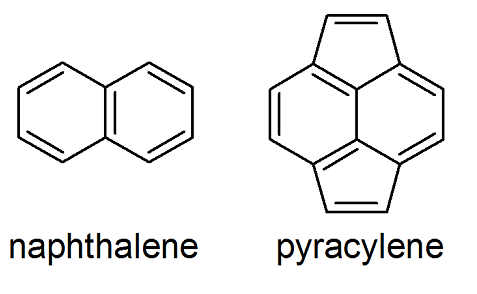
\includegraphics[width=90mm]{polycyclic.png}
\caption{Napthalene has two benzene rings with 2 carbon atoms in common. Even in complex polycylic hydrocarbons such as pyracylene, every ring shares only 2 carbon atoms.}
\label{fig:polycyclic}
\end{figure}

The geometry of ring connectivity is also restrictive. For example, it is not possible for a cycle of length 5 to attach to both rings in pentalene. A cycle of length 5 can only attach to at most one other cycle of length 5. There are some other similar restrictions to add here.

\subsubsection{Huckel's Rule}

Due to the filling of quantum-mechanical electron orbitals, some polycyclic hydrocarbons may be anti-aromatic and therefore extremely unstable. This is commonly known as Huckel's rule in monocyclic molecules. However, we choose to ignore Huckel's rule (and any extensions to multi-cyclic molecules) since anti-aromatic compounds such as pentalene can be stabilized by adding appropriate substituents. Either electron-donating or electron-withdrawing groups can be attached to the ring to allow aromaticity (see Figure ~\ref{fig:pentalene}). Additionally, it is possible to insert hereroatoms into the structure, such as nitrogen or sulphur.

\begin{figure}[ht!]
\centering
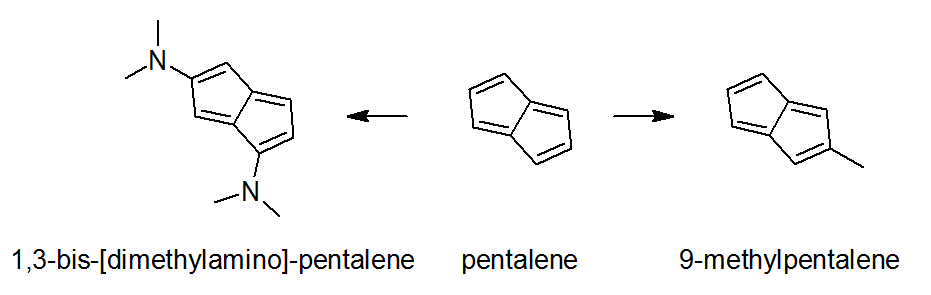
\includegraphics[width=160mm]{pentalene.png}
\caption{Pentalene can attach either the electron-donating Me \cite{methylPentalene} or N(Me)$_2$ \cite{nitrogenPentalene} group to achieve aromatic structure.}
\label{fig:pentalene}
\end{figure}

Finally, graphs representing molecules must be connected. A disjoint graph more accurately represents two molecules rather than one. 

These restrictions prevent the large majority of unrealistic graphs. Our restrictions make no attempt to ensure all graphs can be synthesized. 

\section{Obtaining Realistic Graphs}

We used 4 primary methods to obtain realistic graphs for each Kekule cell, including random, template molecules, graph modification, and a genetic algorithm. All methods limit their graphs to a maximum of 30 nodes. Resulting graphs are converted to SMILES (cite here) (small molecular input line entry system) in order to be visualized. The ports are labeled by atoms with a P (normally reserved for a phosphorous atom). We need not label each port individually since Kekul\'e cells are invariant across port renaming \cite{H13}. The open source Chemistry Development Kit \cite{CDK} is used to parse the SMILES and generate a two-dimensional structure. Other than the ports, the structure resembles the hydrogen-suppressed carbon skeleton of the molecule.  

\subsection{Template Molecules}

Ports were placed at all possible combinations in many known polycyclic aromatic hydrocarbons. The resulting graph was tested for its Kekule cell. Molecules used includes Benzene, Napthalene, Azulene, Acenaphthylene, Pyracylene, Biphenyl, Anthracene, Phenanthrene, and Pyrene.

\subsection{Modification}

Graphs obtained by Hesselink \cite{H13} were modified through a series of cell-invariant operations to meet our restrictions. 

\subsubsection{Cycle Extension and Contraction}
Cycle extension is done by inserting two additional carbon atoms into the cycle at the same position (see Figure ~\ref{fig:cycleExtension}). This has no effect on the Kekul\'e cell as the two atoms are conjugated with the rest of the ring and simply expand it. This procedure is nearly identical to operation v of \cite{v06}. Care must be taken to not select two nodes which also are a part of another cycle, as the resulting graph will contain unrealistic bonding distances and cycle connectivity. The opposite procedure can be used to contract cycles.

\begin{figure}[ht!]
\centering
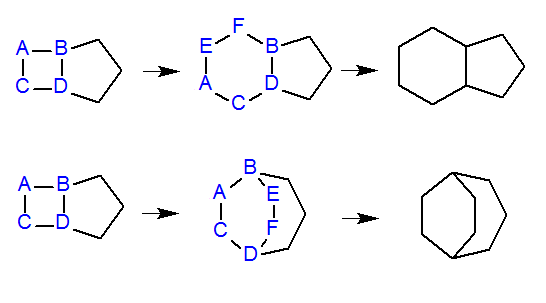
\includegraphics[width=90mm]{cycleExtension.png}
\caption{This shows the extension of the left 4 cycle into a proper 6 cycle. The top half shows a correct procedure, selecting to add nodes between A and B. The bottom half shows the incorrect procedure of adding two nodes in between B and D. Double bonds are excluded from this diagram for clarity.}
\label{fig:cycleExtension}
\end{figure}

\subsubsection{Connecting a Disjoint Graph}
A disjoint graph is not an accurate representation of a single molecule. Luckily, disjoint graphs can often be connected using the following procedure. Internal verticies are added which always conjugate ’within’ themselves, and therefore do not interfere with the cell. For example, see Figure ~\ref{fig:disjoint}.

\begin{figure}[ht!]
\centering
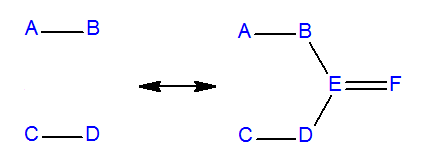
\includegraphics[width=90mm]{disjoint2.png}
\caption{Process used to turn a disjoint graph to a connected graph with the same cell. Two new nodes E and F can be added which always conjugate to each other.}
\label{fig:disjoint}
\end{figure}

In the right-hand graph of Figure ~\ref{fig:disjoint}, F is not a port and so must always contain a double bond. The only other node which is available to form a double bond with F is E, so in every resonance structure of this molecule E and F will contain a double bond with each other (as shown in right diagram). Therefore D or B can never form a double bond with their new added edge (that would result in two adjacent double bonds), and the Kekul\'e cell has not been changed. This procedure is similar to Operation iii and vi of [3].

\subsubsection{Split a Node}

Hesselink et. al \cite{HH13} described a method for splitting a node of high degree into multiple nodes of lower degree. 

\subsection{Genetic Algorithm}

A genetic algorithm is used to search for graphs which apply to a given cell. The algorithm begins by randomly generating a population of graphs. In each iteration, the survivors of last generation's population must be chosen. This is done by selecting the best performing graphs (fitness-wise), along with a smaller amount of random graphs. Random graphs are added to ensure genetic diversity in the population. This sub-population now undergoes genetic operations such as mutation and crossover. 

\subsubsection{Mutation}

Mutation involves randomly perturbing graphs to obtain new ones. Mutations include:
\begin{enumerate}
\item Addition of a node
\item Removal of a random node, and all edges to it
\item Addition of a random edge \footnote{ Edges are randomly chosen until an edge is found that can be added without breaking our restrictions on the degree of vertices.}
\item Removal of a random edge
\item Port Extension
\end{enumerate}

Port extension involves adding a new node in the position of every port, and then adding the port connected to that node. This is often useful for spreading the ports out and allowing new edges without breaking our degree restrictions. This is not guaranteed to preserve the Kekule Cell. See Figure ~\ref{fig:portExtension}.

\begin{figure}[ht!]
\centering
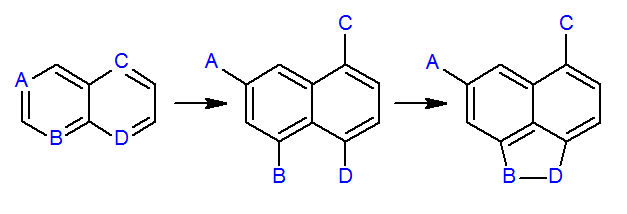
\includegraphics[width=110mm]{portExtension.png}
\caption{Napthalene (left) undergoing a port extension (center). Notice that after the port extension, it is now feasible to add an edge between B and D, which can then create Acenaphthene (right).}
\label{fig:portExtension}
\end{figure}

\subsubsection{Crossover}

Crossover begins by randomly selecting 2 graphs from the sub-population. These graphs are combined to create a new child graph. Children receive all edges which both parents share, and have a 50\% chance to get any other edge found in one of the parents. This creates children which are a hybrid of both their parents.

\subsubsection{Fitness Function}

Fitness values are integers given to a graph. Any graph's cell can be calculated using Hesselink's procedure \cite{H13}. The fitness is calculated by iterating over the graphs cell compared to the cell we are evolving towards. For every port assignment they share, the fitness is incremented by one. For every port assignment that is missing, or is extra, fitness is decremented one point. 

\section{Results}

Realistic Graphs for all cells of rank 4 and 5 have been found. Hesselink was able to find graphs with no restrictions for 210 out of 214 cells with rank 6 \cite{H13}. None of our methods were able to find graphs, realistic or not, for the 4 missing cells of rank 6. We compare the performance of each of our methods based on cells of rank 6 (see Table 1).

Table 1. The amount of Kekule cells of rank 6 that each method was able to find realistic graphs for, according to our restrictions.
\begin{center}
	
  \begin{tabular}{ | l | r |}
    \hline
    Methodology & Cells of Rank 6 Found \\
    \hline
    Template Molecules & 44 \\
    Graph Modification & 32 \\
    Random Graphs & 135 \\
    Genetic Algorithm & 70 \\
    \hline
  \end{tabular}
\end{center}

It seems stochastic methods yield the best results for generating realistic graphs from arbitrary ones. As the Kekule cell number increases (K1 - K214), the graphs get more complex. In total we have found realistic graphs for 165 out of 214 graphs, with most of these clustering towards the beginning. See WEBSITE for a full table.

It would be interesting to see more cell-invariant operations. Not only would this improve the raw modification method, but unrealistic graphs from other methods may also be able to be modified. It would also be interesting to discover to what extent this class of molecules is synthesizable. 

Polycylic aromatic hydrocarbons are commonly produced as byproducts of fuel burning, and have been classified as carcinogenic, mutagenic, and teratogenic. This could pose a challenge if we wish to use large aromatic hydrocarbons in circuitry. 

Below is an example of some of our obtained graphs for each Kekule cell of rank 4 and 5.

\clearpage

\begin{figure}[ht!]
\centering
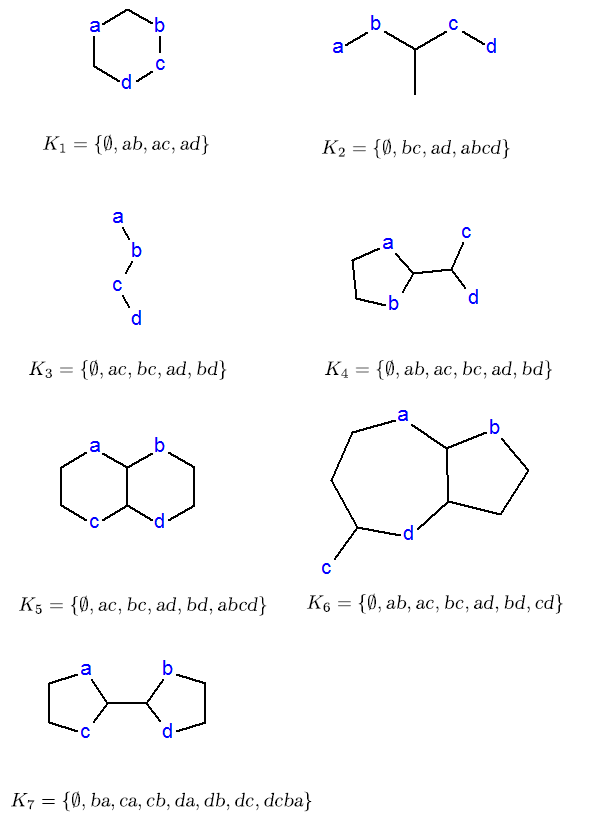
\includegraphics[width=130mm]{rank4Results.png}
\caption{Realistic Graphs for each cell in Hesselink's classification of all cells with rank 4. K$_1$ resembles benzene, K$_5$ napthalene, and K$_6$ azulene.}
\label{fig:rank4Results}
\end{figure}

\begin{figure}[ht!]
\centering
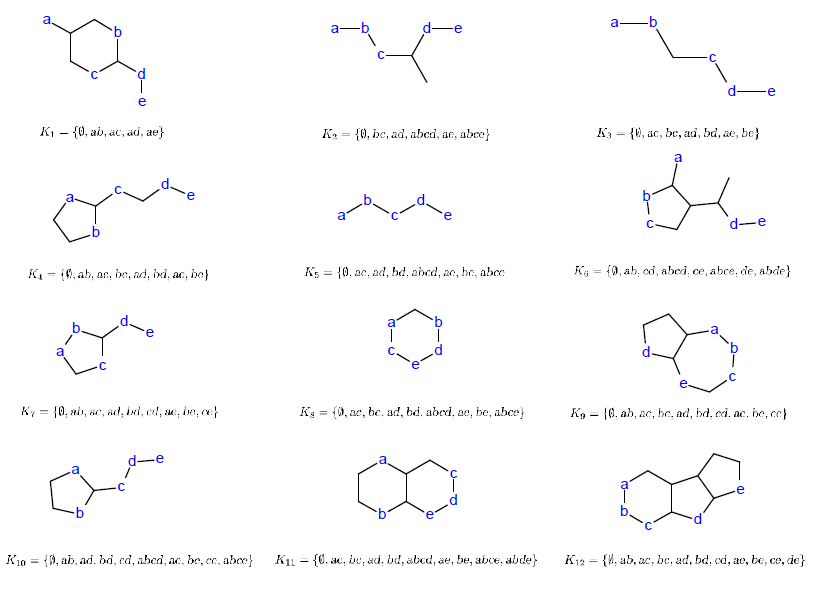
\includegraphics[width=160mm]{rank5Results1.png}
\caption{Realistic Graphs for the first 12 cells in Hesselink's classification of all cells with rank 5. K$_1$ and K$_8$ resembles benzene, K$_{11}$ napthalene, and K$_9$ azulene.}
\label{fig:rank5Results1}
\end{figure}

\begin{figure}[ht!]
\centering
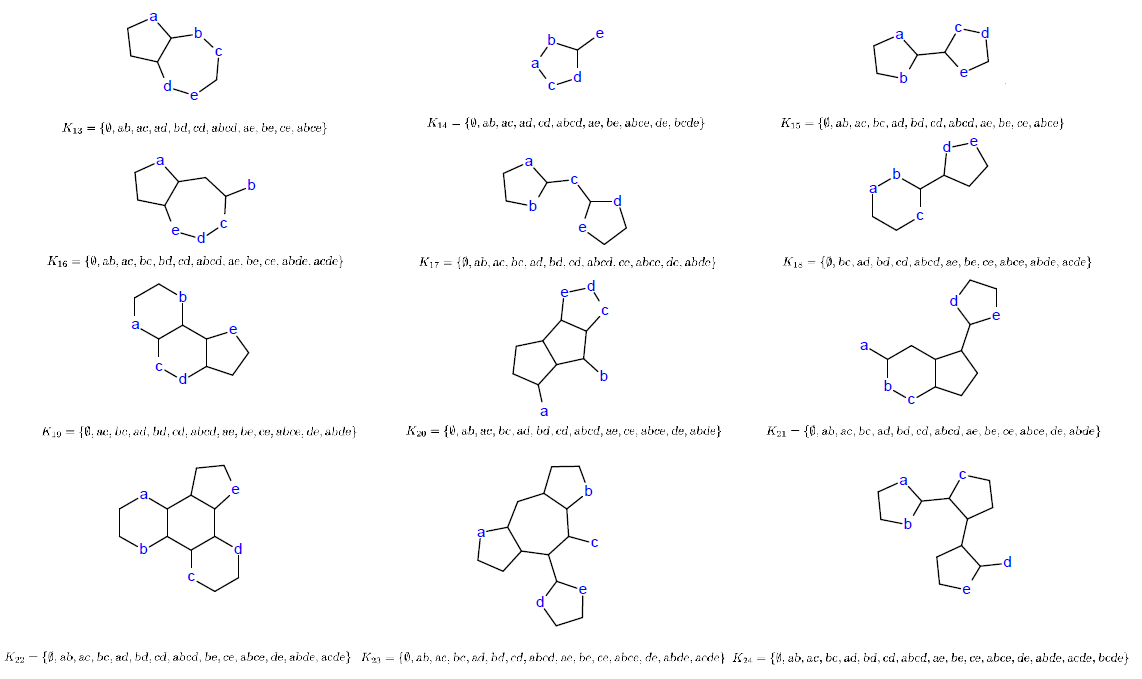
\includegraphics[width=160mm]{rank5Results2.png}
\caption{Realistic Graphs for the second half of cells in Hesselink's classification of all cells with rank 5. K$_{13}$, K$_{16}$ azulene both resemble azulene.}
\label{fig:rank5Results2}
\end{figure}

\begin{thebibliography}{abrv}

\bibitem{H13} W. H. Hesselink, Graph Theory for alternating hydrocarbons with attached ports. Indagationes Mathematicae, Elsevier, 24:115141, 2013.
\bibitem{HH13} W.H. Hesselink, J.C. Hummelen, H.T. Jonkman, H.G. Reker, G.R. Renardel de Lavalette, M.H. van der Veen, Kekule Cells for Molecular Computation. Cornell University Library Online, 2013.
\bibitem{v06} M.H. van der Veen. $\pi$-Logic. PhD thesis, University of Groningen, May 2006.
\bibitem{HK88} A.J. Heeger, S. Kivelson, J.R. Schrieffer, and W.-P Su. Solitons in conducting polymers, Rev. Mod. Phys.,60:781, 1988.
\bibitem{Moore} G. E. Moore, Cramming more components onto integrated circuits. Electronics Magazine. p. 4. Retrieved 2006-11-11. 
\bibitem{CDK} Steinbeck, Christoph, et al. "The Chemistry Development Kit (CDK): An open-source Java library for chemo-and bioinformatics." Journal of chemical information and computer sciences 43.2 (2003): 493-500.
\bibitem{MooreEnd} C. A. Mack, Fifty Years of Moore's Law. IEEE Transactions on semiconductor manufacturing, 24:2 2011.
\bibitem{OmniConj} M. H. van der Veen, M. T. Rispens, H. T. Jonkman, and J. C. Hummelen, Molecules with Linear $\pi$-Conjugated Pathways between all Substituents: Omniconjugation. Adv. Function Mater, 14:3, 2004.
\bibitem{openPath} S.N. Yalirahi, M.A. Ratner, Interplay of topology and chemical stability on the electronic transport of molecular junctions, Ann. New York Acad. Sci. 960 (2002) 153.
\bibitem{9} J. Reichert, R. Ochs, D. Beckmann, H. B. Weber, M. Mayor, H. von Löhneysen,Phys. Rev. Lett. 2002, 88, 176804. 
\bibitem{10} A. Aviram, M. A. Ratner, Chem. Phys. Lett. 1974, 29, 277.
\bibitem{11} D. B. Strukov, K. K. Likharev, Nanotechnology 2005, 16, 137.
\bibitem{12} Y. Karzazi, J. Cornil, J. L. Brédas, J. Am. Chem. Soc. 2001, 123, 10076.
\bibitem{13} J. M. Tour, M. Kozaki, J. M. Seminario, J. Am. Chem. Soc. 1998, 120, 8486.
\bibitem{14} A. Aviram, J. Am. Chem. Soc. 1988, 110, 5687.
\bibitem{15} H. W. Ch. Postma, T. Teepen, Z. Yao, M. Grifoni, C. Dekker, Science 2001, 293, 76.
\bibitem{16} C. Joachim, J. K. Gimzewski, Chem. Phys. Lett. 1997, 265, 353.
\bibitem{17} T. D. Anthopoulos, C. Tanase, S. Setayesh, E. J. Meijer, J. C. Hummelen, P. W. M. Blom, D. M. de Leeuw, Adv. Funct. Mater. 2004, 16, 2174.
\bibitem{18} G. M. Tsivgoulis, J.-M. Lehn, Chem. Eur. J. 1996, 2, 1399.
\bibitem{19} J. J. D. de Jong, L. N. Lucas, R. M. Kellogg, J. H. van Esch, B. L. Feringa, Science 2004, 304, 278.
\bibitem{20} A. P. de Silva, H. Q. N. Gunaratne, C. P. McCoy, Nature 1993, 364, 42.
\bibitem{21} F. M. Raymo, S. Giordani, J. Org. Chem. 2003, 68, 4158.
\bibitem{22} K. Rurack, A. Koval'chuck, J. L. Bricks, J. L. Slominskii, J. Am. Chem. Soc. 2001, 123, 6205.
\bibitem{23} D. Parker, J. A. G. Williams, Chem. Commun. 1998, 245.
\bibitem{24} A. P. de Silva, I. M. Dixon, H. Q. N. Gunaratne, T. Gunnlaugsson, P. R. S. Maxwell, T. E. Rice, J. Am. Chem. Soc. 1999, 121, 1393.

\bibitem{HuckelBad} Roberts, J. D., Streitwieser Jr, A., and Regan, C. M. Small-Ring Compounds. X. Molecular Orbital Calculations of Properties of Some Small-Ring Hydrocarbons and Free Radicals. Journal of the American Chemical Society, 74(18), 4579-4582. 1952.

\bibitem{HuckelExtension} Kruszewski, J., and Krygowski, T. M. An Extension of the Hückel 4N+ 2 Rule to Polycyclic Non-alternant Conjugated Hydrocarbons. Canadian Journal of Chemistry, 53(6), 945-951. 1975.

\bibitem{methylPentalene} Hafner, K., Donges, R., Goedecke, E. and 
Kaiser, R. Concerning Pentalene, 2-Methylpentalane, and 1,3-
Dimethylpentalene. Angew. Chem. Int. Ed. Engl., 12: 337-339. 1973.

\bibitem{nitrogenPentalene} Hafner, K., Bangert, K. F. and Orfanos, V 1,3-Bis(dimethylamino)pentalene. Angew. Chem. Int. Ed. Engl., 6: 451–452. 1967.

\end{thebibliography}

\end{document}
